\begin{frame}
	\frametitle{氢弹的\textrm{Teller–Ulam}构型}
美国的``Teller–Ulam''构型是世界上最早的氢弹构型\\
    \vspace{-0.3cm}
    \begin{figure}
        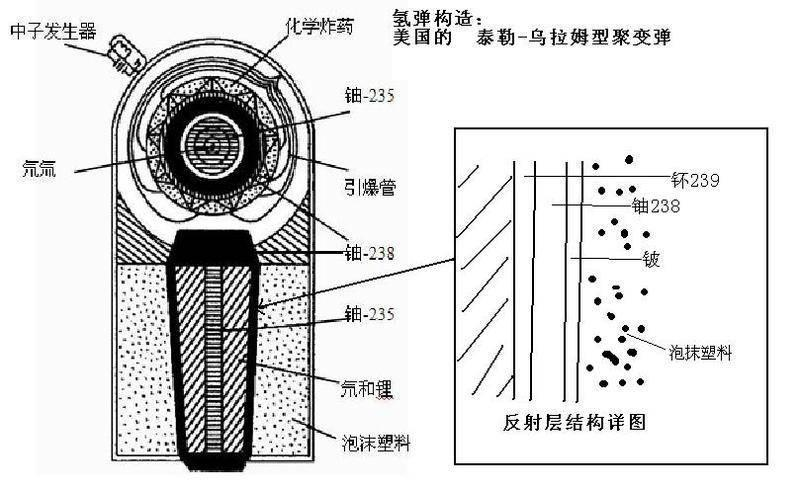
\includegraphics[width=0.8\textwidth]{Figures_History/U-T_design.jpg}
    \end{figure}
		``Teller–Ulam''构型的氢弹采用两级炸弹结构,存在保存养护成本高、体积大等缺点
\end{frame}

\begin{frame}
    \frametitle{中国氢弹的核心突破}
    20世纪60年代,国际上对氢弹技术严密封锁,于敏、黄祖洽等科学家在艰难条件下,独立开展氢弹原理和构型的研究\\
    通过他们的努力,我国仅用2年8个月就成功完成从原子弹到氢弹的跨越,相比其他国家,大大缩短了研发时间
    \begin{itemize}
        \item 材料创新:~使用固态氘化锂作为热核燃料,解决了传统液氚燃料储存和维护难题,极大提高了氢弹的稳定性和可靠性
        \item 独特设计:~我国氢弹的构型采用的物理设计,巧妙利用原子弹爆炸产生的辐射,更高效地压缩和点燃聚变材料,提升核聚变反应效率
        \item 小型化优势:~在同等当量下,我国氢弹的体积更小、重量更轻,便于搭载和投放,增强了武器的机动性和实用性
    \end{itemize}
\end{frame}

\begin{frame}
    \frametitle{氢弹的引爆}
%    \textbf{引爆方式}
    \vspace{-0.4cm}
    \begin{figure}
        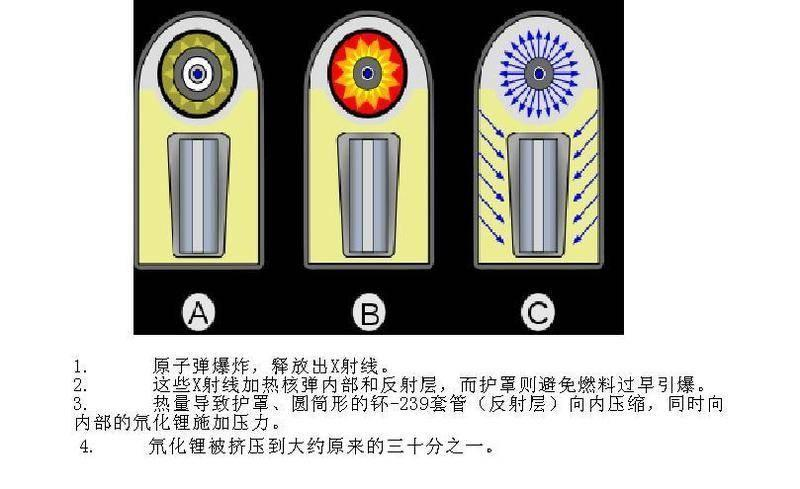
\includegraphics[width=0.8\textwidth]{Figures_History/U-T_design-2.jpg}
    \end{figure}
    氢弹需借助原子弹作为``扳机''来启动核聚变反应:
    \begin{enumerate}
        \item 原子弹引爆:\\
		{\fontsize{7.2pt}{4.2pt}\selectfont{触发原子弹内的核裂变反应,释放出强烈的光辐射、\textrm{X}射线和高能粒子流}}
        \item 辐射内爆:\\
		{\fontsize{7.2pt}{4.2pt}\selectfont{强辐射与粒子流作用于氢弹的聚变材料,使其迅速升温、增压,形成向心的内爆过程,压缩聚变材料}}
        \item 核聚变启动:\\
		{\fontsize{7.2pt}{4.2pt}\selectfont{在超高温、超高压环境下,氢的同位素发生聚变反应,释放出更为巨大的能量,其威力通常远超作为``扳机''的原子弹}}
    \end{enumerate}
\end{frame}

\begin{frame}
    \frametitle{战略核武器小型化}
重要意义
    \begin{itemize}
	    \item \textcolor{magenta}{提升机动性:}\\
		{\fontsize{6.2pt}{4.2pt}\selectfont{小型化的战略核武器,体积和重量大幅减小,可搭载于多种平台,如导弹、潜艇、战机等,显著增强了核力量的机动性与灵活性,能够实现快速部署与打击}}
	\item \textcolor{magenta}{增强突防能力}\\
		{\fontsize{6.2pt}{4.2pt}\selectfont{体积更小的核弹头,有助于降低被敌方探测和拦截的概率,提升核打击的有效性和可靠性}}
	\item \textcolor{magenta}{降低成本}\\
		{\fontsize{6.2pt}{4.2pt}\selectfont{减少核材料和其他组件的使用量,在保证核威慑力的同时,降低了研发、生产和维护成本}}
    \end{itemize}
%    \vspace{0.5cm}
实现途径
    \begin{itemize}
        \item 优化设计:\\
		{\fontsize{6.2pt}{4.2pt}\selectfont{通过改进核弹头的结构设计,%如采用更紧凑的核反应装置和更高效的引爆系统,在不降低爆炸威力的前提下,减小核弹头的体积和重量\\
		%以新型内爆式结构设计为例,能够更精准地控制核反应过程,
		提高核材料的利用率}}
        \item 新材料应用:\\
		{\fontsize{6.2pt}{4.2pt}\selectfont{研发和使用新型材料,%如高强度、低密度的结构材料,以及性能更优异的核材料,
		减轻核弹头的重量,提高其性能和可靠性}}
    \end{itemize}
%    \vspace{0.5cm}
%    \textbf{中国成就}
    我国在战略核武器小型化领域取得了显著成就,不仅提升了我国核力量的现代化水平,也为维护国家安全和世界和平做出了重要贡献
%    \vspace{0.5cm}
%    \begin{figure}
 %       %此处可插入中国小型化战略核武器或相关运载平台的示意图片
 %       \caption{中国小型化战略核武器成果}
 %   \end{figure}
\end{frame}

%\begin{frame}
%    \frametitle{总结}
%    今天我们回顾了“两弹”的研发历程,认识了伟大的两弹元勋,探索了原子弹和氢弹背后的科学原理,领略了于敏构型的独特魅力,以及战略核武器小型化的成就。“两弹”精神将激励我们为中华民族伟大复兴不懈奋斗!
%    \vspace{0.5cm}
%    \begin{figure}
%        \includegraphics[width=0.8\textwidth]{collective_photo.jpg}
%    \end{figure}
%\end{frame}
